\documentclass[black,white]{beamer}

\usepackage{beamerthemesplit}
\usepackage{epstopdf}
\usepackage{graphicx}
\usepackage{subfigure}
\usepackage{hyperref}
\usepackage[utf8]{inputenc}
\usepackage[english]{babel}
\usepackage{listings}
\usepackage{array}
\usepackage{color}
\usepackage{colortbl}

\usefonttheme{professionalfonts}
\usecolortheme{dove}
\useoutertheme{infolines}
\useinnertheme{rectangles}

\setlength{\parindent}{0pt}
\newcommand*\sfb[1]{\textbf{#1}}
\definecolor{red2}{rgb}{.7,0,.39}
\definecolor{grey}{rgb}{0.5,0.5,0.5}
\setbeamercolor{title}{fg=white}
\setbeamercolor{frametitle}{fg=white}
\setbeamercolor{framesubtitle}{fg=white}
\setbeamercolor{normal text}{fg=white}
\setbeamercolor{itemize item}{fg=white}
\setbeamercolor{itemize subitem}{parent=itemize item}
\usebackgroundtemplate{
	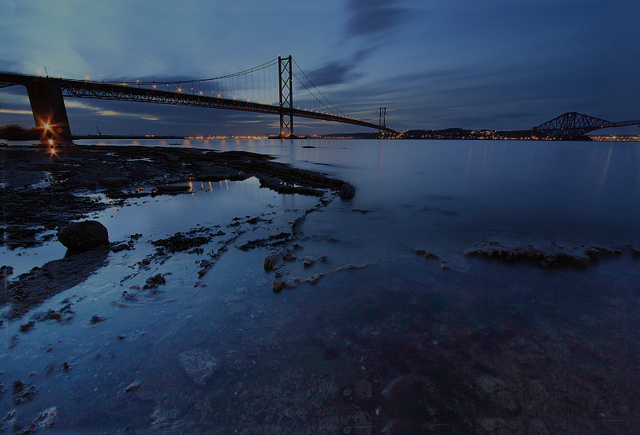
\includegraphics[width=\paperwidth,height=\paperheight]{img/bg.jpg}
}
\setbeamertemplate{footline}%{infolines theme}
{
\leavevmode%
\hbox{%
\begin{beamercolorbox}[wd=.333333\paperwidth,ht=2.25ex,dp=1ex,center]{author in head/foot}%
\usebeamerfont{author in head/foot}\insertshortauthor%~~(\insertshortinstitute)
\end{beamercolorbox}%
\begin{beamercolorbox}[wd=.333333\paperwidth,ht=2.25ex,dp=1ex,center]{title in head/foot}%
\usebeamerfont{title in head/foot}\insertshorttitle
\end{beamercolorbox}%
\begin{beamercolorbox}[wd=.333333\paperwidth,ht=2.25ex,dp=1ex,right]{date in head/foot}%
\usebeamerfont{date in head/foot}\insertshortdate{}\hspace*{2em}
\insertframenumber{} / \inserttotalframenumber\hspace*{2ex}
\end{beamercolorbox}}%
\vskip0pt%
}

\begin{document}

\title[On creating a novel telephony network]{\huge{On creating a novel global telephony network}}
\author[Daniel Borkmann] {
	\vspace*{-20pt}
	\newline
	Daniel Borkmann	\texttt{<dborkma@tik.ee.ethz.ch>}\\
	\texttt{http://gnumaniacs.org}\\\bigskip
	IET PATW 2011, Switzerland
}
\date[\today]{}

\frame {
	\titlepage
}

\frame {
	\frametitle{Some notes about myself}
	\begin{itemize}
		\item 2006-2009: Technical Computer Science, B. Sc., HTWK Leipzig\medskip
		\item Since 2009: Computer Science, M. Sc., HTWK Leipzig\medskip
		\item Since 2009: Scholarship from the German National Merit Foundation\medskip
		\item Since 2011: Master thesis, ETH Zurich\medskip
		\item Software development as a student worker and in my spare time\medskip
		\begin{itemize}
			\item Siemens, Max Planck Society, ipoque\medskip
			\item RoboCup, several Open Source projects
		\end{itemize}
	\end{itemize}
}

\frame {
	\frametitle{Situation among todays telecommunications industry}
	\begin{itemize}
		\item Oligopoly, i.e. approx 10 providers in Switzerland [1]\medskip
		\item Cost issues especially on international calls\medskip
		\item Proprietary legacy systems with security flaws [2]\medskip
		\item Privacy issues, i.e. wiretapping, censorship [3]\medskip
		\item Sparsely in focus of university research
	\end{itemize}
}

\frame {
	\frametitle{\textcolor{grey}{How others tried to challenge this:} \\ 1) Skype}
	\begin{itemize}
		\item Implements VoIP, looks as an alternative on the first hand, but ...\medskip
		\item Almost everything is obfuscated, many antidebugging tricks, much ciphered code (Is there something to hide ?) [4]\medskip
		\item Impossible to scan for trojan/backdoor/malware inclusion [4]\medskip
		\item RC4 is used for obfuscation not for privacy [4]\medskip
		\item Counter-productiveness to its user base [5] [10]\
	\end{itemize}
}

\frame {
	\frametitle{\textcolor{grey}{How others tried to challenge this:} \\ 2) GoogleTalk/GoogleVoice}
	\begin{itemize}
		\item Also implements VoIP, proprietary like Skype\medskip
		\item No end-to-end encryption [6]\medskip
		\item Not usable by hardware phones\medskip
		\item Google seems to save your human voice for other purposes [7]\medskip
		\item Needs Adobe Flash Player (''Symantec recently highlighted Flash for having one of the worst security records in 2009.'') [8]
	\end{itemize}
}

\frame {
	\frametitle{\textcolor{grey}{How we can challenge this:} \\ Basic requirements for a new global telephony network}
	\begin{itemize}
		\item Use of a robust underlying and widespread network \textcolor{green}{$\rightarrow$ VoIP, Internet}\medskip
		\item Compatibility with hardware phones \textcolor{green}{$\rightarrow$ SIP}\medskip
		\item Openness/transparency of the system \textcolor{green}{$\rightarrow$ Open Source}\medskip
		\item No call fees/charges \textcolor{green}{$\rightarrow$ Only for Internet access}\medskip
		\item Strong cryptography between endpoints \textcolor{green}{$\rightarrow$ i.e. ECC, McEliece}\medskip
		\item Control by users instead of companies \textcolor{green}{$\rightarrow$ Open Source Community}\medskip
	\end{itemize}
}

\frame {
	\frametitle{Design of the telephony network architecture}
	\begin{itemize}
		\item Software should run on an \textbf{embedded system} and consists of 4 parts\medskip
		\begin{itemize}
			\item \textbf{SIP server} for communication with trusted phones in LAN\medskip
			\item \textbf{D}istributed \textbf{H}ash \textbf{T}able for global participant retrieval\medskip
			\item \textbf{Client/Server} for voice transmission via Internet\medskip
			\item Internal \textbf{address book} for participant namespace translations
		\end{itemize}
	\end{itemize}
	\hspace*{15pt}
	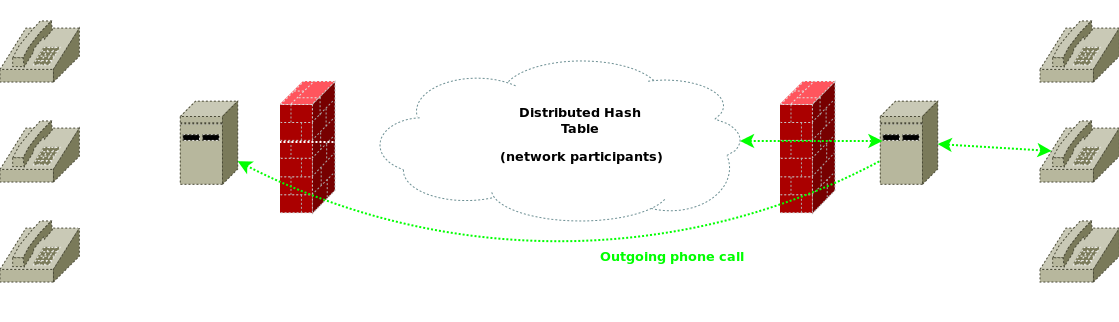
\includegraphics[width=0.9\textwidth]{img/scheme.png}
}

\frame {
	\frametitle{Design of the telephony network architecture}
	\begin{itemize}
		\item \textbf{Distributed Hash Table} (DHT, i.e. Kademlia [9]): \\\medskip $f(\text{User}):=[\text{IP}_{\text{public}}, \text{Port}_{\text{public}}]$, \textit{where} $\text{User}:=SHA_{256}(\text{Key}_{\text{public}})$\medskip
		\item Internal \textbf{address book}: \\\medskip $g(\text{PhoneNumber}):=\text{Username}$ \textit{and} $h(\text{Username}):=\text{Key}_{\text{public}}$\medskip
		\item \textbf{Connection endpoint}: \\\medskip $f(SHA_{256}(h(g(\text{PhoneNumber}))))$\medskip
		\item Voice information is then \textbf{encrypted} with $\text{Key}_{\text{public}}$\medskip
		\item Ideally, the client/server protocol cannot be recognized by ISPs DPIs\medskip
		\item ($\text{IP}_{\text{public}}, \text{Port}_{\text{public}}$ obtained via STUN)
	\end{itemize}
}

\frame {
	\frametitle{Scenario: Bob calls Alice}
	\begin{enumerate}
		\item Both parties have exchanged their $\text{Key}_{\text{public}}$ (once)\medskip
		\item Bob calls i.e. $1234$ from his SIP phone, where $g(1234)$:=\texttt{Alice}\medskip
		\item Since \texttt{Alice} has a registered public key, $h(\text{\texttt{Alice}}):=\text{Key}_{\text{Alice,public}}$\medskip
		\item Bob looks up $SHA_{256}(\text{Key}_{\text{Alice,public}})$ by applying to $f$ in the DHT\medskip
		\item Bob receives $[\text{IP}_{\text{Alice,public}}, \text{Port}_{\text{Alice,public}}]$\medskip
		\item Bob opens a direct and $\text{Key}_{\text{Alice,public}}$-encrypted connection to Alice\medskip
		\item Alice accepts the connection from Bob, delivers a notification to her SIP phones and both parties transfer their encrypted voice data
	\end{enumerate}
}

\frame {
	\frametitle{Conclusion}
	\begin{itemize}
		\item By the distributed manner, the network is more stable towards outages\medskip
		\item Through openness of the system, wide range of research and audits can be performed\medskip
		\item System is privacy-enhanced and "resistant" against wiretapping\medskip
		\item Compatiblity to a wide range of SIP hardware phones for easy usage
	\end{itemize}
}

\frame {
	\frametitle{}
	\bigskip
	\bigskip
	\begin{center}
		\Large{Thanks for your attention! Questions?}\\
		\bigskip
		\bigskip
		\bigskip
		\bigskip
		\texttt{dborkma@tik.ee.ethz.ch}\\
		\medskip
		\texttt{http://gnumaniacs.org}
	\end{center}
}

\frame {
	\frametitle{References, 24.05.2011}
	\begin{itemize}
		\item [1] \url{http://www.telecomrating.ch/ratingaktuell.html}
		\item [2] \url{http://events.ccc.de/congress/2010/Fahrplan/events/4208.en.html}
		\item [3] \url{http://www.zdnetasia.com/beware-govts-are-tapping-your-3g-calls-62201577.htm}
		\item [4] \url{http://www.blackhat.com/presentations/bh-europe-06/bh-eu-06-biondi/bh-eu-06-biondi-up.pdf}
		\item [5] \url{http://www.nartv.org/mirror/breachingtrust.pdf}
		\item [6] \url{http://tinyurl.com/3l9pzrf}
		\item [7] \url{http://cartesianproduct.wordpress.com/2011/05/02/google-wants-your-voice/}
		\item [8] \url{http://www.apple.com/hotnews/thoughts-on-flash/}
		\item [9] \url{http://www.gnumaniacs.org/kademlia.pdf}
		\item [10] \url{http://slashdot.org/story/11/05/24/2010222/Microsoft-Kills-Skype-For-Asterisk}
	\end{itemize}
}

\end{document}

